
\documentclass[a4paper,10pt,12pt]{article}%
\usepackage{float}
\usepackage{amssymb}
\usepackage{amsmath}
\usepackage{amsfonts}
\usepackage{graphicx}
\usepackage{epstopdf}
\usepackage{theorem}
\usepackage[onehalfspacing]{setspace}%
\setcounter{MaxMatrixCols}{30}
\addtolength{\textwidth}{3cm}
\addtolength{\hoffset}{-1.5cm}
\addtolength{\textheight}{2cm}
\addtolength{\voffset}{-1cm}
\newtheorem{theorem}{Theorem}
\newtheorem{acknowledgement}[theorem]{Acknowledgement}
\newtheorem{algorithm}[theorem]{Algorithm}
\newtheorem{axiom}[theorem]{Axiom}
\newtheorem{case}[theorem]{Case}
\newtheorem{claim}[theorem]{Claim}
\newtheorem{conclusion}[theorem]{Conclusion}
\newtheorem{condition}[theorem]{Condition}
\newtheorem{conjecture}[theorem]{Conjecture}
\newtheorem{corollary}{Corollary}
\newtheorem{criterion}[theorem]{Criterion}
\newtheorem{definition}{Definition}
\newtheorem{example}[theorem]{Example}
\newtheorem{exercise}[theorem]{Exercise}
\newtheorem{lemma}{Lemma}
\newtheorem{notation}[theorem]{Notation}
\newtheorem{problem}[theorem]{Problem}
\newtheorem{proposition}{Proposition}
{
\theorembodyfont{\rmfamily}
\newtheorem{remark}[theorem]{Remark}
}
\newtheorem{solution}[theorem]{Solution}
\newtheorem{summary}[theorem]{Summary}
\newenvironment{proof}[1][Proof]{\noindent\textbf{#1.} }{\ \rule{0.5em}{0.5em}}
\begin{document}


\def\symbolfootnote[#1]#2{\begingroup%
\def\thefootnote{\fnsymbol{footnote}}\footnote[#1]{#2}\endgroup} 

\renewcommand\baselinestretch{1.6}
\small\large\normalsize

\begin{center}


{\LARGE Problem Set 6 }\\[0.6cm]
{\large   EC 588, Spring 2015 } 


{\large Due by 22/05/2015}\\[1.0cm]

Submitted by\\
{\Large Suat Akbulut} 
\footnote{E-mail: zubuat@gmail.com} \\[0.6cm]


{ABSTRACT}

\end{center}
{\small  This  homework aims to improve the command over numerical dynamic programming through studying 
heterogeneous-agent incomplete market models by considering the Huggett (1993) environment. When coefficient of relative risk aversion is 1.5 and credit limit is set to -2, we conclude that the equilibrium bond price is $0.9911$, which yields an interest rate of $0.8\%$ interest rate in contrast to Table 1 in Huggett (1993) but, consistent with the real data. The paper calculates the decision rules and stationary distrubition of agents as well as gini coefficient since heterogeneity of the individual creates inequality in income distribution and, lastly, it concludes with welfare loss of uninsurable environment  . } \\[0.4cm]


{\bf Keywords:} MATLAB,  Heterogeneous-Agent Incomplete Market Model, Huggett (1993), Value Function Iteration, Binary Search Model, ... .

{\bf Jel Classification:} ... , ... 


\newpage


\section*{Introduction}
 
 This paper tries to replicate the Huggett's (1993) heterogeneous-agent incomplete market environment. In his environment:
 \begin{itemize} 
\item While households are hit by unemployment shocks, there are no aggregate shocks hitting the economy, hence given that at the steady-state the distribution of households are time-invariant and constant over asset and shock state pairs, the aggregate variables, such as total endowment, consumption; and prices, such as the price of bonds are time invariant, and constant, as well. 
\item Households do not have access to Arrow-Debreu securities to insure themselves against unemployment shocks. Instead, there is only a single type of non-contingent (risk-free) bond that pays 1 unit next period, which is traded this period at a price of $q$. Note that, this arrangement can be considered a bond that pays at a net real interest rate of r units, where the return satisfies $q=\frac{1}{1+r}$.
\item By generating sufficient impatience, $\frac{\beta}{q}<1$, we restrain unbounded capital accumulation motive of households.
\end{itemize}
In such environment, the problem of a household born with $(s,a)$ state levels is the following:
\begin{align*}
V(s,a) =  \underset{ a' \in A }{\text{max}}
 & \left\lbrace u\left[ y(s) + a - qa' \right] + \beta \sum_{s' \in S} \pi(s'|s) \cdot V(s',a')  \right\rbrace
\end{align*}
where $a'$ satisfies 
\begin{align*}
\underline{a} \leq a' \leq \frac{y(s)+a}{q}
\end{align*}
where
\begin{align*}
\underline{a} > \underline{a}^{NBL} = - \frac{y(u)}{1-q}
\end{align*}

Following is the Algorithm that we will be following to solve the above problem by help of MATLAB.
\section*{Algorithm}
To solve the model numerically, the algorithm we employ is as follows:
\begin{enumerate}
\item Start with an initial guess for the bond price $q^0$ such that $\beta < q^0 < 1$.
\item Given $q^0$, solve households's problem using value function iteration to obtain $a'=g(s,a;q^0)$.
\item Using the obtained decision rule and the exogenous law of motion of the idiosyncratic shocks, derive the stationary distribution by iterative application. Define the fixed point as $\mu^0(s,a;q^0)$.
\item Compute $A^0$. If $A^0=0$ you are done, you found the equilibrium! If $A^0 \neq 0$, the price cannot clear the market, and we need to set a new price that clears the good and the asset markets. If $A^0<0$, there is not enough demand for the bond, and we need to raise the return so as to make the bond more attractive, which means we need to reduce its price, $q^0$. If $A^0>0$, there is too much demand for the bond, so we need to decrease the return from the bond, or in other words, we need to increase its price,$q^0$. After updating the price, we return to step 2, and go over the same steps until we find the price at which markets clear.
\end{enumerate}
While updating the $q$, I will makes use of the binary search algorithm. That is to say I will keep updating the interval that $q$ must be fall in. By doing so I will narrow the interval band from $1-\beta$ to $ \frac{1-\beta}{2^k}$ after k iteration. 

\section*{Parameters and Functional Forms}
Let the parameter values and functional forms be as follows: The discount factor $\beta=0.96$, coefficient of relative risk aversion $\alpha=1.5$ with a power utility function $u(c)=\frac{c^{1-\alpha}}{1-\alpha}$, the set of possible earnings $S=\{e,u\}$ where $y(e) = 1$ and $y(u) = 0.1$ are interpreted as earnings when employed (normalized to unity) and unemployed respectively, the Markovprocess for earnings $\pi(s'=e|s=e)=0.80$ and $\pi(s'=u|s=u)=0.50$, and the space of asset holdings be given by the compact set $A=[-2,5]$.
\section*{Results}

\begin{figure}[H]
\centering
   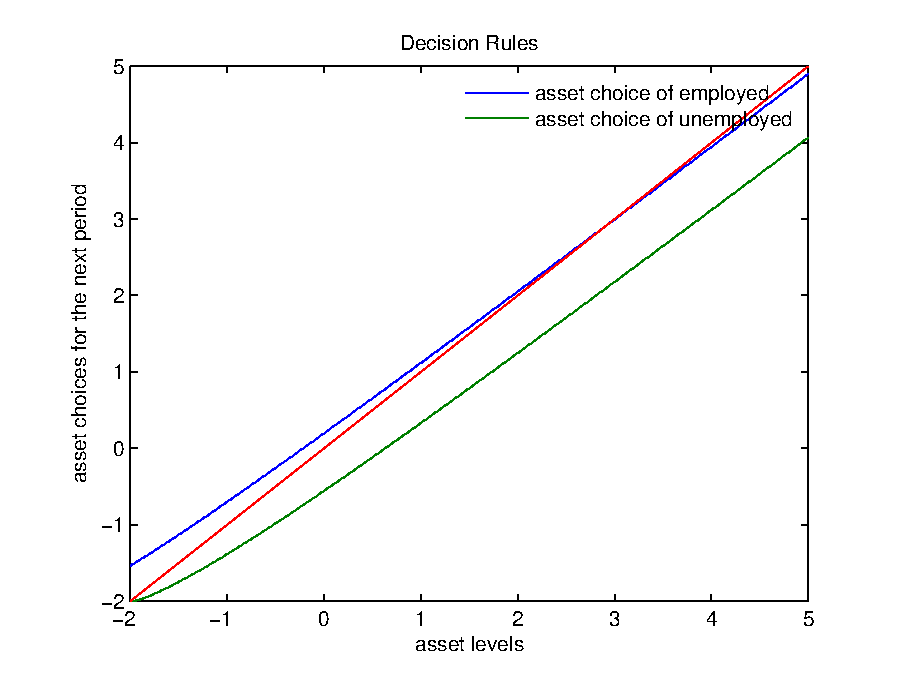
\includegraphics[scale=1]{assetchoice.eps} 
  \begin{center}
   \caption{Decision rule for the employed and unemployed states }
   \label{apolicy}
  \end{center}
\end{figure}
Having derived the decision rule $g(s,a;q^*)$ by the use of value function iteration, Figure \ref{apolicy} illustrates the optimal asset holding rule for employed and unemployed state. As in Figure 1 of Huggett (1993), only the decsion rule for employed state intersects the $45$ line. But the intersection occurs at a different point. That is because transition matrix of Markov Process is differ in the sense that probability of an employed individual being employed in the next period is higher in Huggett (1993).\footnote{In this paper we assume $\pi(s'=e|s=e)=0.80$, however, Huggett (1993) uses 0.925 for this probability.} As expected, both value function and decision rule is always above for the employed state.
\begin{figure}[H]
\centering
   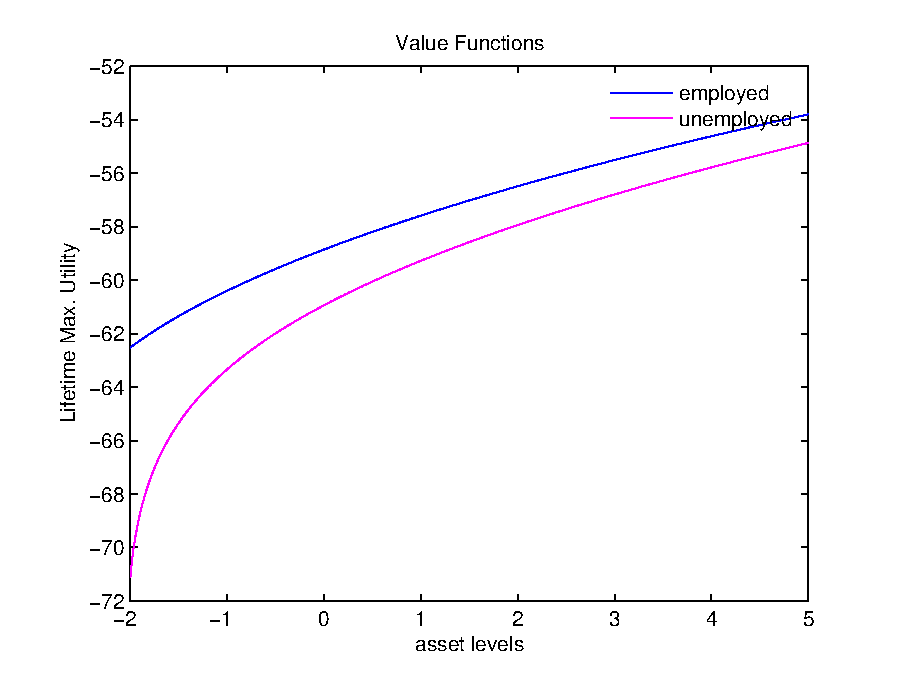
\includegraphics[scale=1]{valuefnc.eps} 
  \begin{center}
   \caption{Value function for the employed and unemployed states }
   \label{value}
  \end{center}
\end{figure}
Using decision rule $g(s,a;q^*)$ and Markovchain probablity matrix $\pi(s'|s)$ we derive the stationary distribution of agents, $\mu(s,a;q^*)$. Figure \ref{stadist} illustrates the distribution og the agents for different $s$ states. And also observe that the upper bound of the asset grid is not binding.
\begin{figure}[H]
\centering
   \includegraphics[scale=1]{stadist.eps} 
  \begin{center}
   \caption{Stationary distribution for employed and unemployed states }
   \label{stadist}
  \end{center}
\end{figure}
By using the decision rules and distribution of agents, we can calculate the level of economy-wide asset holdings, which should be zero in net supply in equilibrium. The results are shown in Table \ref{tab:results}. When coefficient of relative risk aversion, $\alpha$ is 1.5 and, credit limit that we assume, $\underline{a}$, is -2, we find still positive interest rate as opposed to what Huggett (1993) presents in its Table 1. 
\begin{table}[htbp]
  \centering
  \caption{Equilibirum values of bond price, $q$, interest rate, $r$, and economy wide asset holding, $A^0$}
    \begin{tabular}{|c|c|c|}
    \hline
    $q$     & $r$     & $A^0$      \\
    \hline
    \hline
    0.991172 & 0.008907 & 0.000012 \\
    \hline
    \end{tabular}%
  \label{tab:results}%
\end{table}%

By the help a MATLAB code that I found on the web, coded by Yvan Lengwiler, I calculated gini index, which is 0.40503 and, Figure \ref{gini} shows the Lorenz curve that depicts the income inequality in the equilibrium of our economy
\begin{figure}[H]
\centering
   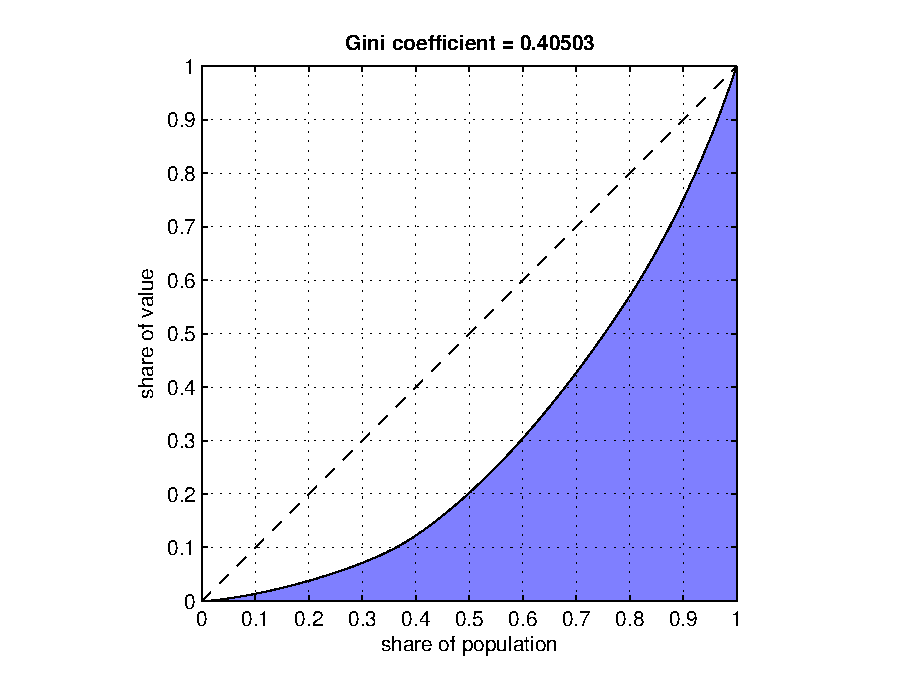
\includegraphics[scale=1]{gini.eps} 
  \begin{center}
   \caption{Gini index and Lorenz Curve}
   \label{gini}
  \end{center}
\end{figure}
In order to find the welfare gain from full insurance, $W^F-W^I$, we must calculate the welfare levels of both situations. Table \ref{tab:welfaregain} shows the corresponding levels and the welfare gain from full insurance.
\begin{table}[htbp]
  \centering
  \caption{Welfare Levels of complete and incomplete markets and, the welfare gain from full insurance}
    \begin{tabular}{|c|c|c|}
    \hline
    $W^F$     & $W^I$     & Welfare Gain      \\
    \hline
    \hline
      -14.5030 &  -59.7133 &  45.2103 \\
    \hline
    \end{tabular}%
  \label{tab:welfaregain}%
\end{table}%
\section*{Conclusion}
In this homework, we replicated the Huggett (1993) environment and had similar results to the original paper. An interest rate of approximately $1\%$ clears the bond market, which is more in line with the real data. We observed that due to the heterogeneity of the individual there is inequality in income distribution. We show that incomplete structure of the market leads a welfare loss. 

\newpage
\begin{thebibliography}{9}

\bibitem{lamport94}
Huggett, M., (1993). "The Risk-Free Rate in Heterogeneous-Agent Incomplete Insurance
Economies", \emph{Journal of Economic Dynamics and Control}, 17, pp. 953-969.

\end{thebibliography}

\end{document}